\section{Comparisons}
This section contains several different comparisons between the different runs to illustrate performance properties of each algorithm. 

\subsection{Making the Comparisons}
Each run of the two algorithms can contain designs that were exposed to numerous different load cases across the possible input space. Additionally, the design results between the Stochastic Loads and the Aggregated LHS methods are not comparaable natively. This is because the Stochastic Loads designs are based on Reliability Index, not peak stress. 

To overcome this inconsistency between the different runs, additional processing was required. The designs from each run were re-analyzed using a single, common reference load of: 

\begin{align*}
P_x &=0\\
P_y &= -147 \text{kN}
\end{align*}

Once the analysis was completed, the peak stress was obtained for each design. This is the data that is presented in the graphs below. Because the load case used to make the data is different from the earlier sections, the stress responses may appear inconsistent with the previous graphs. However, this is due to the change in loading, not because the designs have changed. 

\subsection{Comparison of Long Run Results}
Figure \ref{fig:pfront_comp_long} shows a plot of this compairson between the two Long-Run fronts. Note that the solver for the aggregate LHS appears to cover a wider portion of the solution space, but that both graphs follow roughly the same curve. 

\begin{figure}[!htbp]
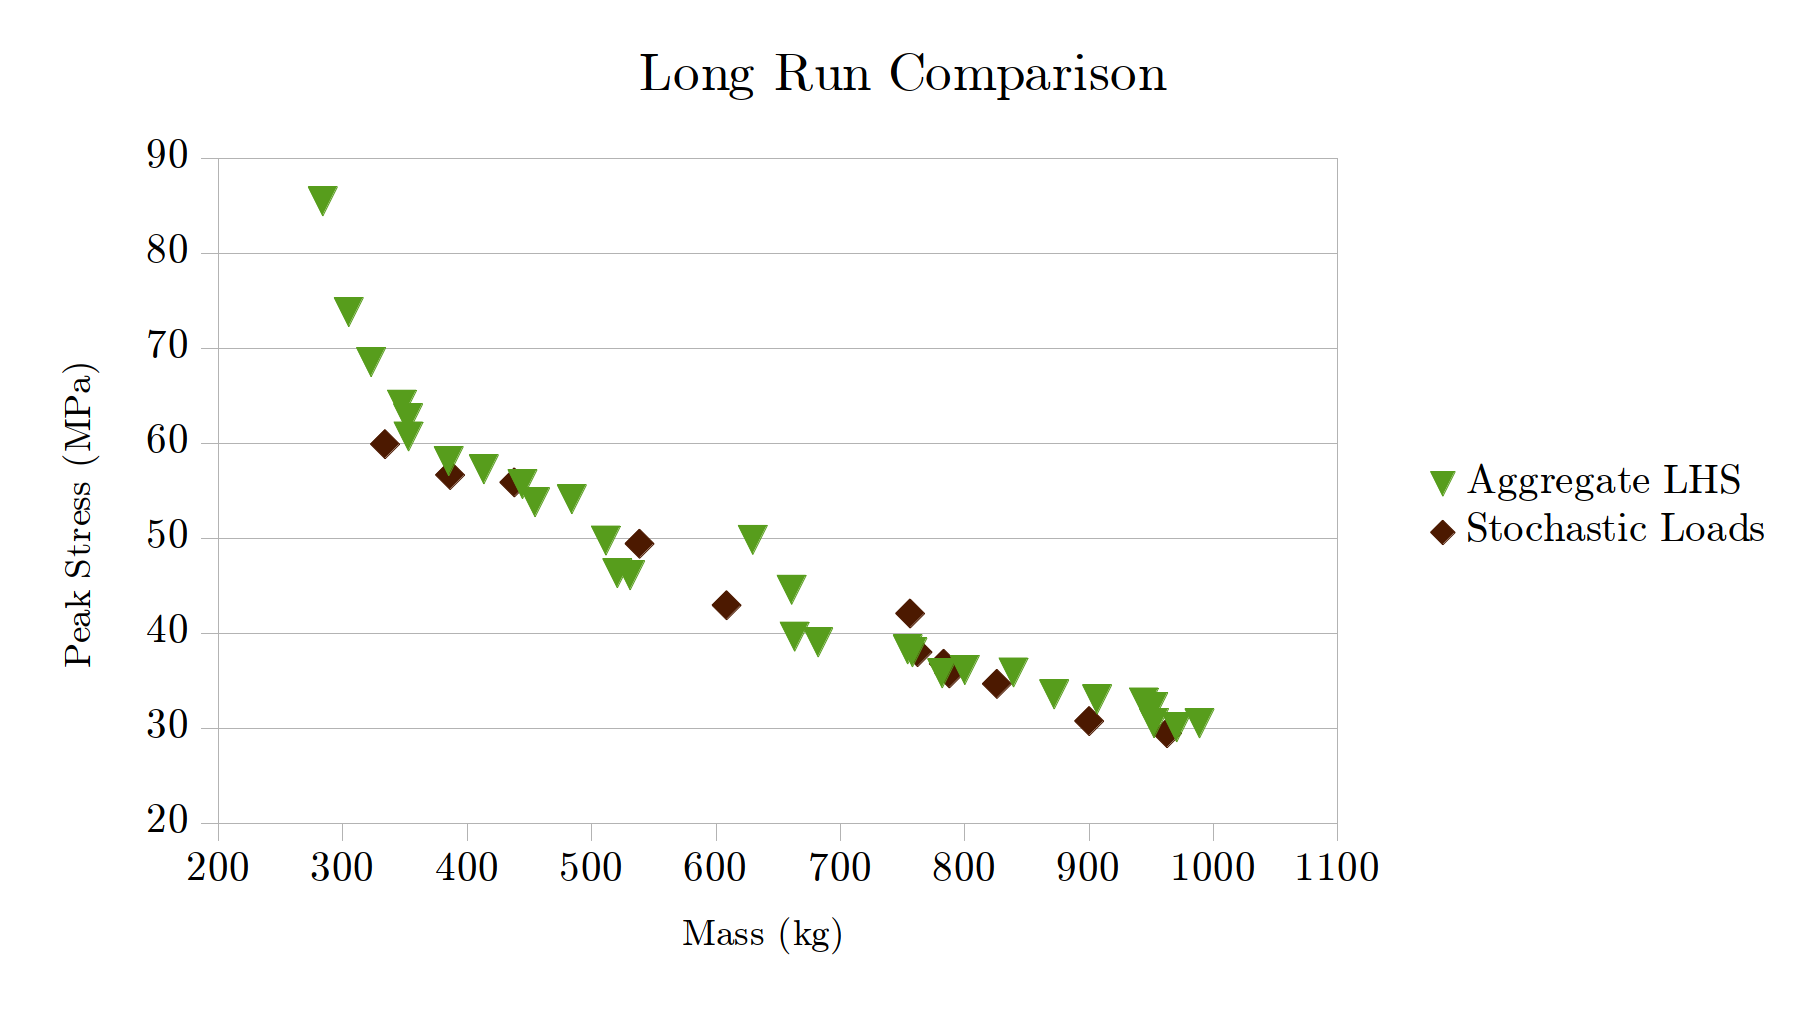
\includegraphics[width=\textwidth]{img/pf_comp_long.png}
\caption{Comparison of the Two Long Run Pareto Plots}
\label{fig:pfront_comp_long}
\end{figure}

\subsection{Comparison of Intermediate Run Results}
Figure \ref{fig:pfront_comp_int} shows a plot of the compairson between the two Intermediate-Run fronts. Note that the solver for the aggregate LHS appears to have slightly better performance at lighter weights than Stochastic Loads. 

\begin{figure}[!htbp]
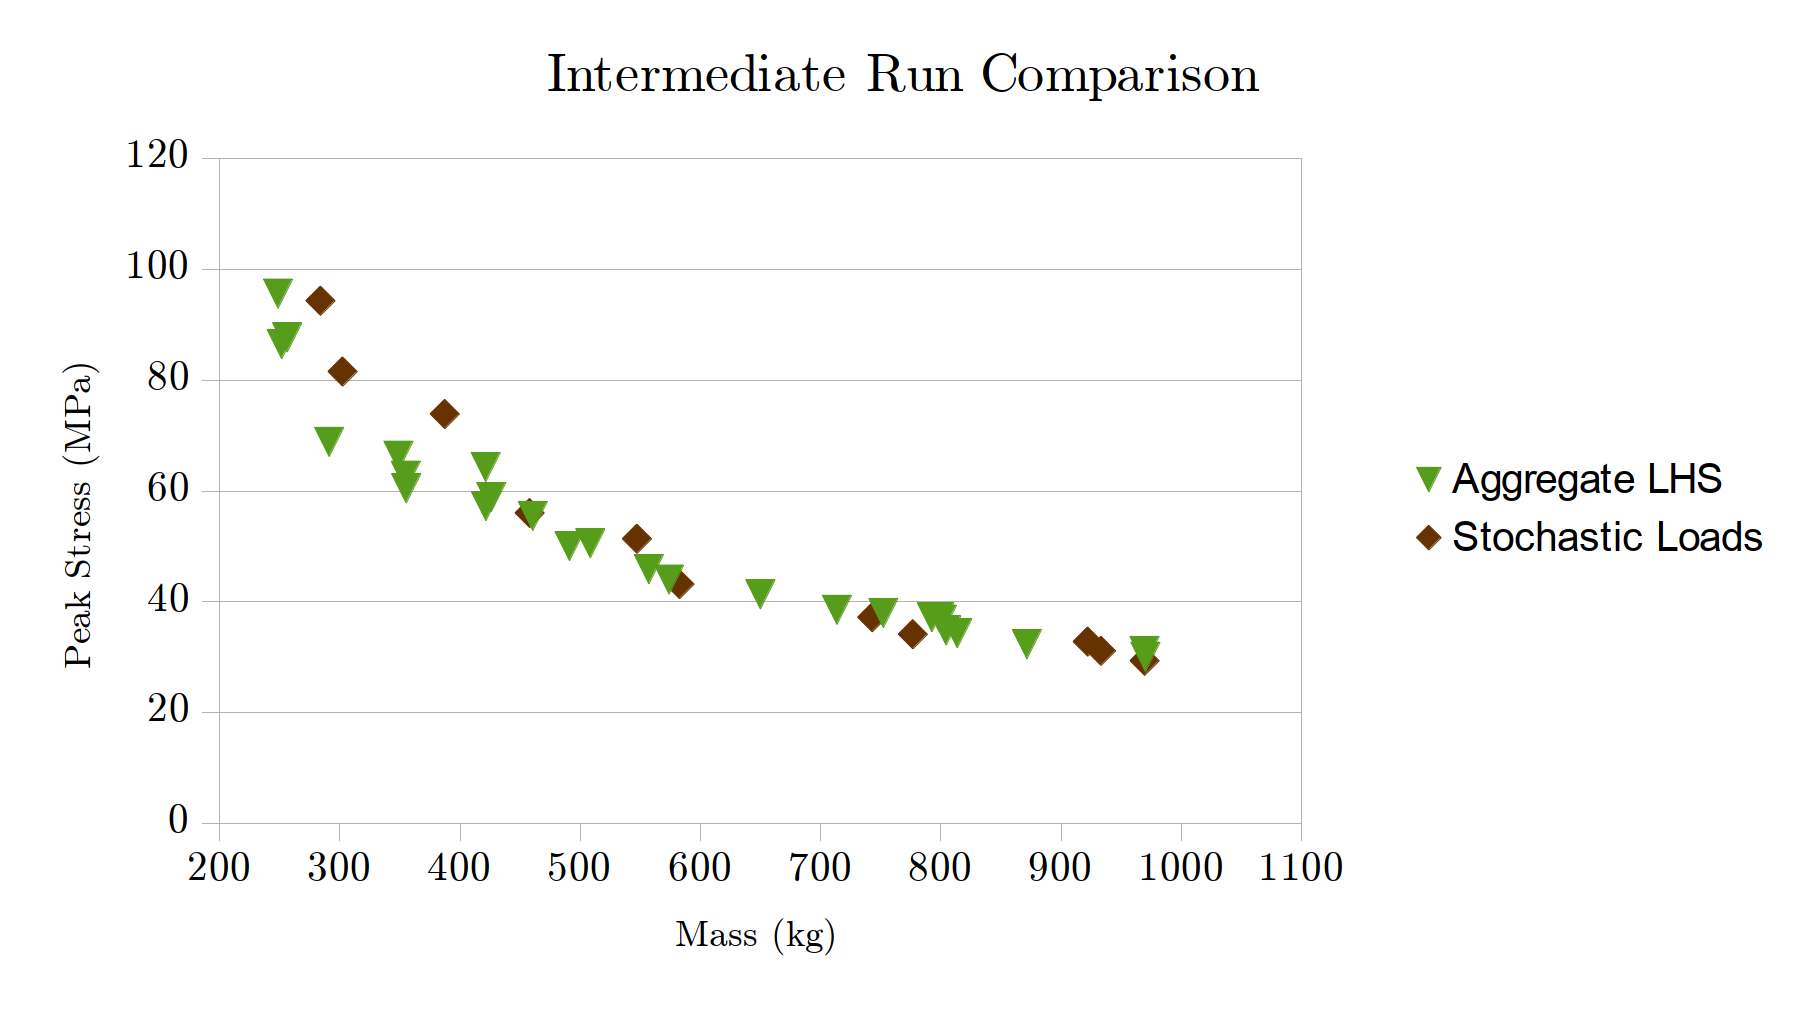
\includegraphics[width=\textwidth]{img/pf_comp_int.png}
\caption{Comparison of the Two Long Run Pareto Plots}
\label{fig:pfront_comp_int}
\end{figure}

\subsection{Comparison of Short Run Results}
Figure \ref{fig:pfront_comp_short} shows a plot of this compairson between the two Short-Run fronts. Note that despite the same solution times, the Stocastic Loads plot has resulted in designs returning higher stress values in some weight ranges. 

\begin{figure}[!htbp]
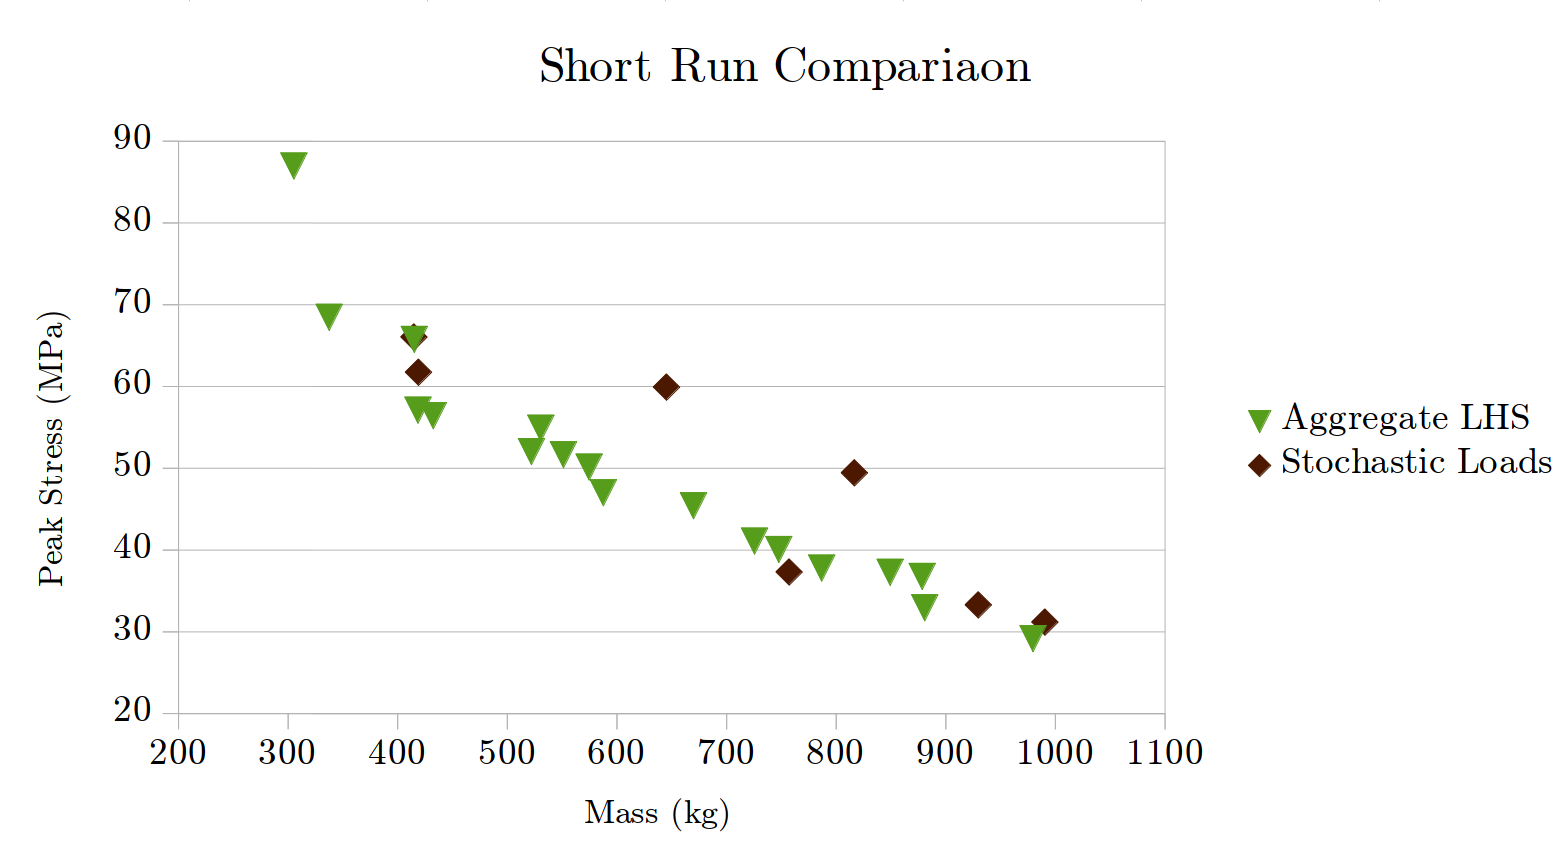
\includegraphics[width=\textwidth]{img/pf_comp_short.png}
\caption{Comparison of the Two Short Run Pareto Plots}
\label{fig:pfront_comp_short}
\end{figure}

\subsection{Comparison of All Stochastic Loads Plots}
Figure \ref{fig:pfront_comp_sto} shows a plot of this compairson between the three Stochastic Loads fronts. Note the increase in accuracy as the solution time rises. 

\begin{figure}[!htbp]
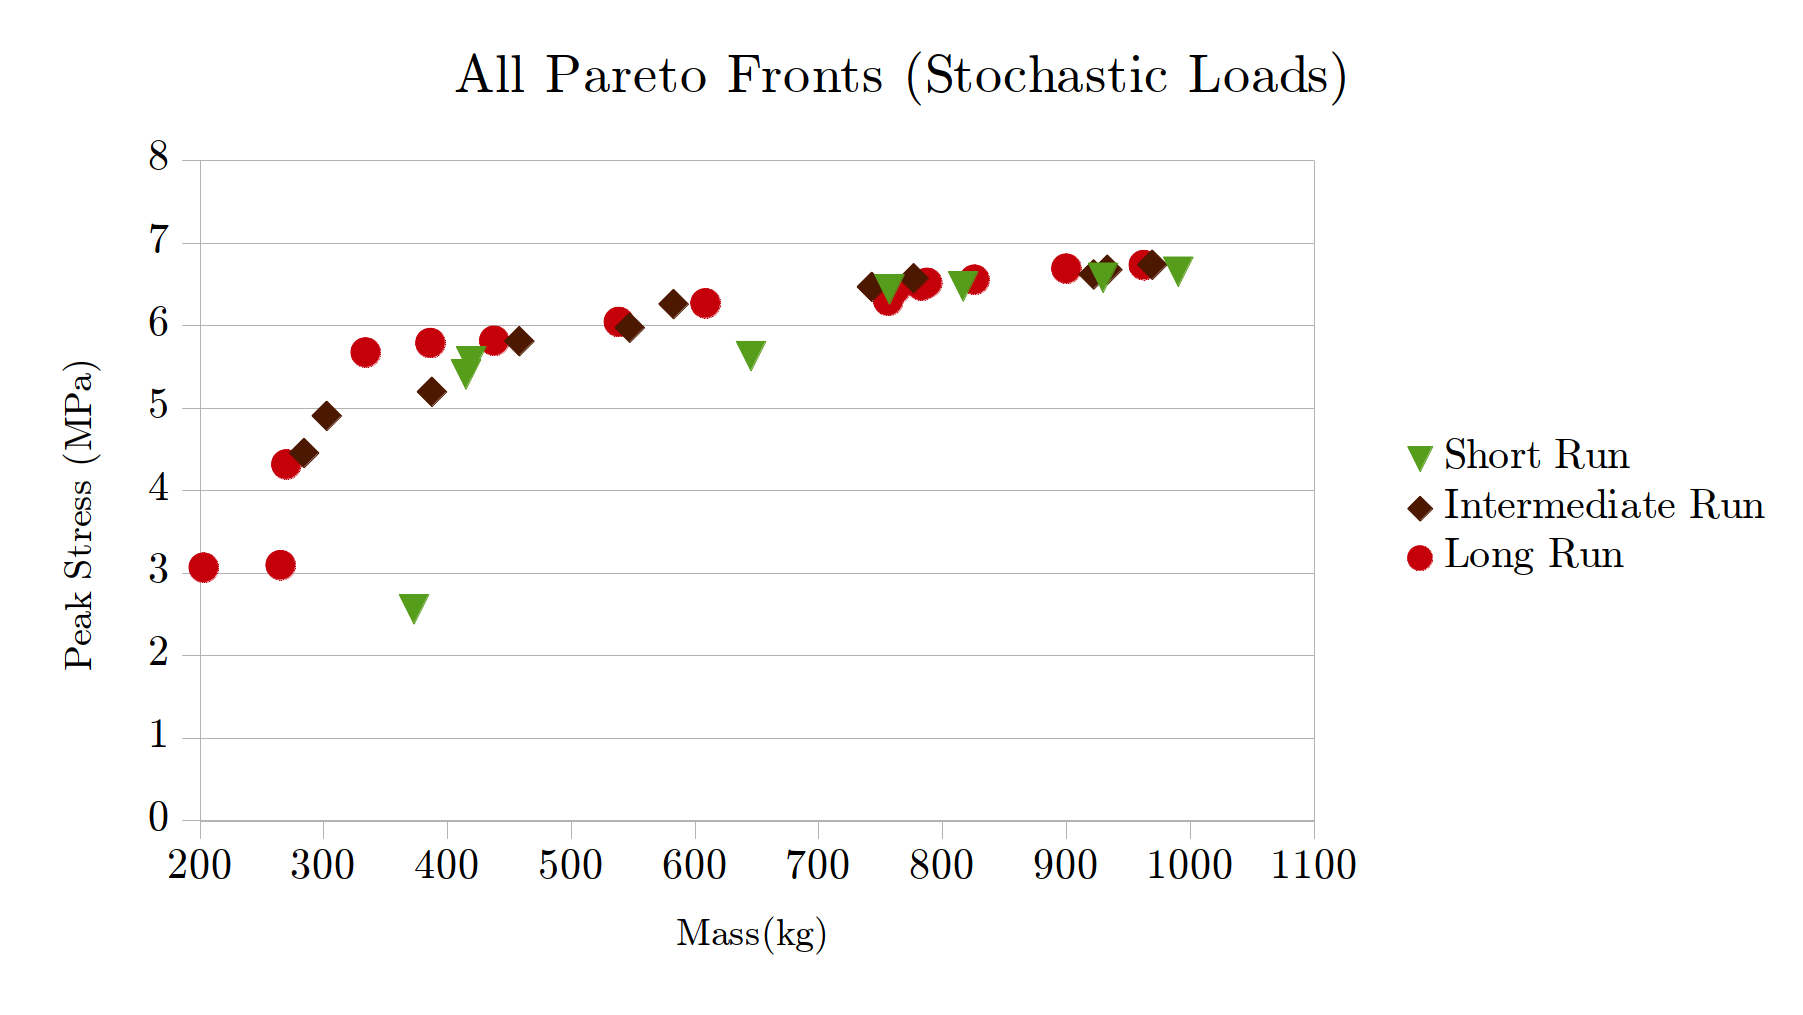
\includegraphics[width=\textwidth]{img/pf_comp_sto.png}
\caption{Comparison of the Stochastic Loads Pareto Plots}
\label{fig:pfront_comp_sto}
\end{figure}

\subsection{Comparison of All Aggregate LHS Plots}
Figure \ref{fig:pfront_comp_agg} shows a plot of this compairson between the three Aggregate LHS fronts. Note the increase in accuracy as the solution time rises, with the exception that the intermediate run seems to have performed better at lighter weights. . 

\begin{figure}[!htbp]
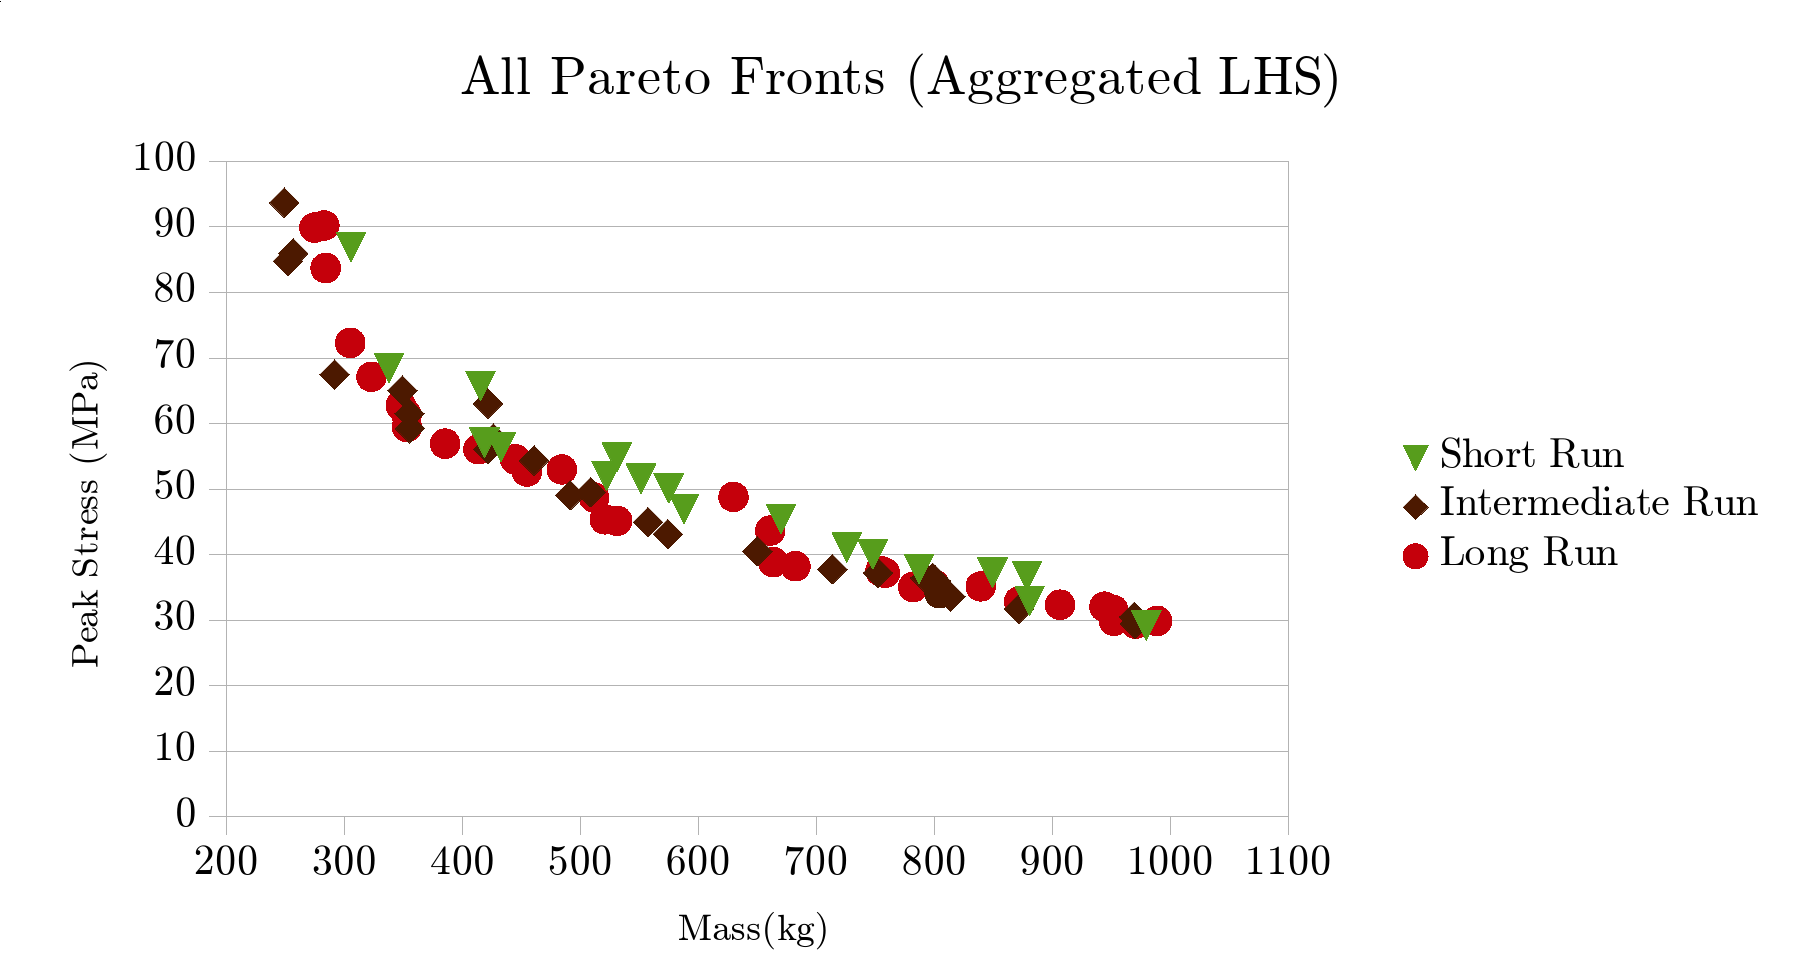
\includegraphics[width=\textwidth]{img/pf_comp_agg.png}
\caption{Comparison of the Aggregate LHS Pareto Plots}
\label{fig:pfront_comp_agg}
\end{figure}
